\documentclass[final,leqno]{siamltex}
\usepackage{lmodern}
\usepackage{amssymb,amsmath}
\usepackage{ifxetex,ifluatex}
\usepackage{fixltx2e} % provides \textsubscript
\ifnum 0\ifxetex 1\fi\ifluatex 1\fi=0 % if pdftex
  \usepackage[T1]{fontenc}
  \usepackage[utf8]{inputenc}
  \usepackage{textcomp} % provides euro and other symbols
\else % if luatex or xelatex
  \usepackage{unicode-math}
  \defaultfontfeatures{Ligatures=TeX,Scale=MatchLowercase}
\fi
% use upquote if available, for straight quotes in verbatim environments
\IfFileExists{upquote.sty}{\usepackage{upquote}}{}
% use microtype if available
\IfFileExists{microtype.sty}{%
\usepackage[]{microtype}
\UseMicrotypeSet[protrusion]{basicmath} % disable protrusion for tt fonts
}{}
\IfFileExists{parskip.sty}{%
\usepackage{parskip}
}{% else
\setlength{\parindent}{0pt}
\setlength{\parskip}{6pt plus 2pt minus 1pt}
}
\usepackage{hyperref}
\hypersetup{
            pdftitle={Ellipsoid Method and Its Amazing Oracles},
            pdfauthor={Wai-Shing Luk},
            pdfkeywords={Ellipsoid method, Cutting plane method, Separation oracle, Cholesky Factorization},
            pdfborder={0 0 0},
            breaklinks=true}
\urlstyle{same}  % don't use monospace font for urls
\usepackage{graphicx,grffile}
\makeatletter
\def\maxwidth{\ifdim\Gin@nat@width>\linewidth\linewidth\else\Gin@nat@width\fi}
\def\maxheight{\ifdim\Gin@nat@height>\textheight\textheight\else\Gin@nat@height\fi}
\makeatother
% Scale images if necessary, so that they will not overflow the page
% margins by default, and it is still possible to overwrite the defaults
% using explicit options in \includegraphics[width, height, ...]{}
\setkeys{Gin}{width=\maxwidth,height=\maxheight,keepaspectratio}
\setlength{\emergencystretch}{3em}  % prevent overfull lines
\providecommand{\tightlist}{%
  \setlength{\itemsep}{0pt}\setlength{\parskip}{0pt}}
\setcounter{secnumdepth}{5}
% Redefines (sub)paragraphs to behave more like sections
\ifx\paragraph\undefined\else
\let\oldparagraph\paragraph
\renewcommand{\paragraph}[1]{\oldparagraph{#1}\mbox{}}
\fi
\ifx\subparagraph\undefined\else
\let\oldsubparagraph\subparagraph
\renewcommand{\subparagraph}[1]{\oldsubparagraph{#1}\mbox{}}
\fi

% set default figure placement to htbp
\makeatletter
\def\fps@figure{htbp}
\makeatother

\ifxetex \usepackage[UTF8]{ctex} \fi
\usepackage{tikz,pgf,pgfplots}
\usepackage{comment}
\usetikzlibrary{arrows}
\definecolor{qqqqff}{rgb}{0.,0.,1.}
\newcommand{\columnsbegin}{}
\newcommand{\columnsend}{}
\newcommand{\col}[1]{}
\newcommand{\pause}{}
\newcommand{\onslide}{}
\usepackage[]{natbib}
\bibliographystyle{plainnat}

\title{Ellipsoid Method and Its Amazing Oracles\thanks{This work was supported by the Society for Industrial and Applied Mathematics}}
\author{Wai-Shing Luk\thanks{Fudan University}}
\date{\today}

\begin{document}
\maketitle
\begin{abstract}
Ellipsoid method is revisited. Besides that, three separation oracles are investigated for applications. They are robust optimization, semidefinite programming, and network optimization. Discuss the stability issue. Finally, the parallel cut is described.
\end{abstract}

\hypertarget{sec:introduction}{%
\section{Introduction}\label{sec:introduction}}

The bad reputation of the ellipsoid method is not good. And that is unfair. It is commonly believed that the method is inefficient in practice for large-scale convex problems. The convergent rate is slow. It cannot exploits sparsity. It was supplanted by the interior-point methods. It can be treated as a theoretical tool for proving the polynomial-time solvability of combinatorial optimization problems.

Nevertheless, the ellipsoid method works very differently compared with the interior point method. Also, it only requires a separation oracle. Thus, it can play nicely with other techniques. Consider Ellipsoid Method When the number of optimization variables is moderate, e.g.~ECO flow, analog circuit sizing, parametric problems. The number of constraints is large, or even infinite. Whenever separation oracle can be implemented efficiently.

\hypertarget{sec:cutting-plane-method-revisited}{%
\section{Cutting-plane Method Revisited}\label{sec:cutting-plane-method-revisited}}

\hypertarget{sec:convex-feasibility-problem}{%
\subsection{Convex Feasibility Problem}\label{sec:convex-feasibility-problem}}

Let \(\mathcal{K} \subseteq \mathbb{R}^n\) be a convex set. Consider the feasibility problem:

\begin{enumerate}
\def\labelenumi{\arabic{enumi}.}
\tightlist
\item
  Find a point \(x^* \in \mathbb{R}^n\) in \(\mathcal{K}\), or
\item
  Determine that \(\mathcal{K}\) is empty (i.e., no feasible solution)
\end{enumerate}

When a \emph{separation oracle} \(\Omega\) is \emph{queried} at \(x_0\), it either

\begin{enumerate}
\def\labelenumi{\arabic{enumi}.}
\tightlist
\item
  Asserts that \(x_0 \in \mathcal{K}\), or
\item
  Returns a separating hyperplane between \(x_0\) and \(\mathcal{K}\):
  \begin{equation}g^\top (x - x_0) + \beta \leq 0, \beta \geq 0, g \neq 0, \; \forall x \in \mathcal{K}.\label{eq:cut}\end{equation}
\end{enumerate}

The pair \((g, \beta)\) is called a \emph{cutting-plane}, or cut, since it eliminates the halfspace \(\{x \mid g^\top (x - x_0) + \beta > 0\}\) from our search. If \(\beta=0\) (\(x_0\) is on the boundary of halfspace that is cut), cutting-plane is called \emph{neutral cut}. If \(\beta>0\) (\(x_0\) lies in the interior of halfspace that is cut), cutting-plane is called \emph{deep cut}.

The \(\mathcal{K}\) is usually given by a set of inequalities \(f_j(x) \le 0\) or \(f_j(x) < 0\) for \(j = 1 \cdots m\), where \(f_j(x)\) is a convex function. A vector \(g \equiv \partial f(x_0)\) is called a \emph{subgradient} of a convex function \(f\) at \(x_0\) if \(f(z) \geq f(x_0) + g^\mathrm{T} (z - x_0)\). Hence, the cut \((g, \beta)\) is given by \((\partial f(x_0), f(x_0))\).

Note that if \(f(x)\) is differentiable, we can simply take \(\partial f(x_0) = \nabla f(x_0)\). Cutting-plane method consists of two key components: separation oracle \(\Omega\) and a search space \(\mathcal{S}\) initially big enough to cover \(\mathcal{K}\). For example,

\begin{itemize}
\tightlist
\item
  Polyhedron \(\mathcal{P}\) = \(\{z \mid C z \preceq d \}\).
\item
  Interval \(\mathcal{I}\) = \([l, u]\) (for one-dimensional problem).
\item
  Ellipsoid \(\mathcal{E}\) = \(\{z \mid (z-x_c)P^{-1}(z-x_c) \leq 1 \}\).
\end{itemize}

Generic Cutting-plane method:

\begin{itemize}
\tightlist
\item
  \textbf{Given} initial \(\mathcal{S}\) known to contain \(\mathcal{K}\).
\item
  \textbf{Repeat}

  \begin{enumerate}
  \def\labelenumi{\arabic{enumi}.}
  \tightlist
  \item
    Choose a point \(x_0\) in \(\mathcal{S}\).
  \item
    Query the cutting-plane oracle at \(x_0\).
  \item
    \textbf{If} \(x_0 \in \mathcal{K}\), quit.
  \item
    \textbf{Else}, update \(\mathcal{S}\) to a smaller set that covers:
    \[\mathcal{S}^+ = \mathcal{S} \cap \{z \mid g^\top (z - x_0) + \beta \leq 0\}.\]
  \item
    \textbf{If} \(\mathcal{S}^+ = \emptyset\) or it is small enough, quit.
  \end{enumerate}
\end{itemize}

\hypertarget{sec:convex-optimization-problem}{%
\subsection{Convex Optimization Problem}\label{sec:convex-optimization-problem}}

Consider:
\begin{equation}\begin{array}{ll}
    \text{minimize}     & f_0(x), \\
    \text{subject to}   & x \in \mathcal{K}.
  \end{array}
\label{eq:convex-optimization}\end{equation}
The optimization problem is treated as a feasibility problem with an additional constraint \(f_0(x) < t\). Here, \(f_0(x)\) could be a convex function or a quasiconvex function. \(t\) is the best-so-far value of \(f_0(x)\). The problem can be reformulated as:
\begin{equation}\begin{array}{ll}
    \text{minimize}   & t, \\
    \text{subject to} & \Phi(x, t) < 0, \\
                      & x \in \mathcal{K},
  \end{array}
\label{eq:cvx-in-feasibility-form}\end{equation}
where \(\Phi(x, t) < 0\) is the \(t\)-sublevel set of \(f_0(x)\). Note that \(\mathcal{K}_t \subseteq \mathcal{K}_u\) if and only if \(t \leq u\) (monotonicity). One easy way to solve the optimization problem is to apply the binary search on \(t\).

Another possible way is, to update the best-so-far \(t\) whenever a feasible solution \(x_0\) is found such that \(\Phi(x_0, t) = 0\). We assume that the oracle takes responsibility for that.

Generic Cutting-plane method (Optim)

\begin{itemize}
\tightlist
\item
  \textbf{Given} initial \(\mathcal{S}\) known to contain \(\mathcal{K}_t\).
\item
  \textbf{Repeat}

  \begin{enumerate}
  \def\labelenumi{\arabic{enumi}.}
  \tightlist
  \item
    Choose a point \(x_0\) in \(\mathcal{S}\)
  \item
    Query the separation oracle at \(x_0\)
  \item
    \textbf{If} \(x_0 \in \mathcal{K}_t\), update \(t\) such that
    \(\Phi(x_0, t) = 0\).
  \item
    Update \(\mathcal{S}\) to a smaller set that covers:
    \[\mathcal{S}^+ = \mathcal{S} \cap \{z \mid g^\top (z - x_0) + \beta \leq 0\} \]
  \item
    \textbf{If} \(\mathcal{S}^+ = \emptyset\) or it is small enough, quit.
  \end{enumerate}
\end{itemize}

\hypertarget{sec:example-profit-maximization-problem}{%
\subsection{Example: Profit Maximization Problem}\label{sec:example-profit-maximization-problem}}

Consider:
\begin{equation}\begin{array}{ll}
   \text{maximize} & p(A x_1^\alpha x_2^\beta) - v_1 x_1 - v_2 x_2, \\
   \text{subject to}& x_1 \le k,
  \end{array}
\label{eq:profit-max-in-original-form}\end{equation}
where
\(p\) is the market price per unit,
\(A\) is the scale of production,
\(p(A x_1^\alpha x_2^\beta)\) is the Cobb-Douglas production function,
\((\alpha, \beta)\) is the output elasticities,
\(x\) is the input quantity,
\(v\) is the output price, and
\(k\) is a given constant that restricts the quantity of \(x_1\).

The formulation is not in the convex form. Rewrite the problem in the following form:
\[\begin{array}{ll}
    \text{maximize}   & t, \\
    \text{subject to} & t  + v_1 x_1  + v_2 x_2 < p A x_1^{\alpha} x_2^{\beta}, \\
                      & x_1 \le k.
  \end{array}
\]
By taking the logarithm of each variable, we have the problem in a convex form:
\begin{equation}\begin{array}{ll}
    \text{max}  & t, \\
    \text{s.t.} & \log(t + v_1 e^{y_1} + v_2 e^{y_2}) - 
                    (\alpha y_1 + \beta y_2) < \log(pA), \\
                & y_1 \le \log k,
  \end{array}
\label{eq:profit-in-cvx-form}\end{equation}
where \(y_1 = \log x_1\), \(y_2 = \log x_2\).

\hypertarget{sec:area-of-applications}{%
\section{Area of Applications}\label{sec:area-of-applications}}

\begin{itemize}
\tightlist
\item
  Robust convex optimization

  \begin{itemize}
  \tightlist
  \item
    oracle technique: affine arithmetic
  \end{itemize}
\item
  Parametric network potential problem

  \begin{itemize}
  \tightlist
  \item
    oracle technique: negative cycle detection
  \end{itemize}
\item
  Semidefinite programming

  \begin{itemize}
  \tightlist
  \item
    oracle technique: Cholesky factorization
  \end{itemize}
\end{itemize}

\hypertarget{sec:robust-convex-optimization}{%
\subsection{Robust Convex Optimization}\label{sec:robust-convex-optimization}}

Consider:
\begin{equation}\begin{array}{ll}
    \text{minimize}   & \sup_{q \in \mathbb Q} f_0(x,q), \\
    \text{subject to} & f_j(x,q) \leq 0, \;
            \forall q \in {\mathbb Q}, \; j = 1,2,\cdots,m,
  \end{array}
\label{eq:robust-optim}\end{equation}
where \(q\) represents a set of varying parameters. The problem can be reformulated as:
\[\begin{array}{ll}
    \text{minimize}   & t, \\
    \text{subject to} & f_0(x,q) < t,  \\
                      & f_j(x,q) \leq 0, \;
            \forall q \in {\mathbb Q}, \; j = 1,2,\cdots,m.
  \end{array}
\]

The oracle only needs to determine:

\begin{itemize}
\tightlist
\item
  If \(f_j(x_0, q) > 0\) for some \(j\) and \(q = q_0\), then
\item
  the cut \((g, \beta)\) = \((\partial f_j(x_0, q_0), f_j(x_0, q_0))\)
\item
  If \(f_0(x_0, q) \geq t\) for some \(q = q_0\), then
\item
  the cut \((g, \beta)\) = \((\partial f_0(x_0, q_0), f_0(x_0, q_0) - t)\)
\item
  Otherwise, \(x_0\) is feasible, then
\item
  Let \(q_{\max} = \text{argmax}_{q \in \mathbb Q} f_0(x_0, q)\).
\item
  \(t := f_0(x_0, q_{\max})\).
\item
  The cut \((g, \beta)\) = \((\partial f_0(x_0, q_{\max}), 0)\)
\end{itemize}

Random sampling trick.

\hypertarget{sec:example-profit-maximization-problem-convex}{%
\subsubsection{Example: Profit Maximization Problem (convex)}\label{sec:example-profit-maximization-problem-convex}}

Consider
\[\begin{array}{ll}
    \text{max}  & t \\
    \text{s.t.} & \log(t + \hat{v}_1 e^{y_1} + \hat{v}_2 e^{y_2}) - 
                        (\hat{\alpha} y_1 + \hat{\beta} y_2) \le \log(\hat{p}\,A)  \\
                & y_1 \le \log \hat{k} .
  \end{array}
\]
Now assume that \(\hat{\alpha}\) and \(\hat{\beta}\) vary \(\bar{\alpha} \pm e_1\) and \(\bar{\beta} \pm e_2\) respectively, where \(\hat{p}\), \(\hat{k}\), \(\hat{v}_1\), and \(\hat{v}_2\) all vary \(\pm e_3\). By detail analysis, the worst case happens when:

\begin{itemize}
\tightlist
\item
  \(p = \bar{p} + e_3\), \(k = \bar{k} + e_3\)
\item
  \(v_1 = \bar{v}_1 - e_3\), \(v_2 = \bar{v}_2 - e_3\),
\item
  if \(y_1 > 0\), \(\alpha = \bar{\alpha} - e_1\), else
  \(\alpha = \bar{\alpha} + e_1\)
\item
  if \(y_2 > 0\), \(\beta = \bar{\beta} - e_2\), else
  \(\beta = \bar{\beta} + e_2\)
\end{itemize}

\begin{quote}
\textbf{Remark}: for more complicated problems, affine arithmetic could be
used.
\end{quote}

\hypertarget{sec:parametric-network-potential-problem}{%
\subsection{Parametric Network Potential Problem}\label{sec:parametric-network-potential-problem}}

Given a network represented by a directed graph \(G = (V, E)\).
Consider:
\[\begin{array}{ll}
    \text{minimize} & t, \\
    \text{subject to} & u_i - u_j \le h_{ij}(x, t), \; \forall (i, j) \in E,\\
    \text{variables} &x, u,
  \end{array}
\]
where \(h_{ij}(x, t)\) is the weight function of edge \((i,j)\).

Assume that the network is large but the number of parameters is small.
Given \(x\) and \(t\), the problem has a feasible solution if and only if \(G\) contains no negative cycle.
Let \(\mathcal{C}\) be a set of all cycles of \(G\). The problem can be formulated as:
\[\begin{array}{ll}
    \text{minimize} & t, \\
    \text{subject to} & W_k(x, t) \ge 0, \forall C_k \in C ,\\
       \text{variables} & x,
\end{array}
\]
where \(C_k\) is a cycle of \(G\):
\[W_k(x, t) = \sum_{ (i,j)\in C_k} h_{ij}(x, t).
\]

The oracle only needs to determine:

\begin{itemize}
\tightlist
\item
  If there exists a negative cycle \(C_k\) under \(x_0\), then
\item
  the cut \((g, \beta)\) = \((-\partial W_k(x_0), -W_k(x_0))\)
\item
  If \(f_0(x_0) \geq t\), then
\item
  the cut \((g, \beta)\) = \((\partial f_0(x_0), f_0(x_0) - t)\)
\item
  Otherwise, \(x_0\) is feasible, then
\item
  \(t := f_0(x_0)\).
\item
  The cut \((g, \beta)\) = \((\partial f_0(x_0), 0)\)
\end{itemize}

\hypertarget{sec:example-optimal-matrix-scaling}{%
\subsubsection{Example: Optimal Matrix Scaling}\label{sec:example-optimal-matrix-scaling}}

Given a sparse matrix \(A = [a_{ij}] \in \mathbb{R}^{N\times N}\).
Find another matrix \(B = U A U^{-1}\) where \(U\) is a nonnegative diagonal matrix, such that the ratio of any two elements of \(B\) in absolute value is as close to 1 as possible.

Let \(U = \mathrm{diag}([u_1, u_2, \ldots, u_N])\). Under the min-max-ratio criterion, the problem can be formulated as:
\[\begin{array}{ll}
    \text{minimize}   &  \pi/\psi  \\
    \text{subject to} &  \psi \leq u_i |a_{ij}| u_j^{-1} \leq \pi, \; 
                                            \forall a_{ij} \neq 0 , \\
                      &  \pi, \, \psi, u, \text{positive} \\
    \text{variables}  &  \pi, \psi, u \, .
  \end{array}
\]

By taking the logarithms of variables, the above problem can be transformed
into:
\[\begin{array}{ll}
    \text{minimize}   &  t \\
    \text{subject to} &  \pi' - \psi' \leq t \\
                      &  u_i' - u_j'  \leq \pi' - a_{ij}', \; \forall a_{ij} \neq 0 \,, \\
                      &  u_j' - u_i' \leq a_{ij}' - \psi', \; \forall a_{ij} \neq 0 \,, \\
    \text{variables}  &  \pi', \psi', u' \, .
  \end{array}
\]
where \(k'\) denotes \(\log( | k | )\) and \(x = (\pi', \psi' )^\top\).

Consider the following problem:
\[\begin{array}{ll}
    \text{minimize}    & t, \\
    \text{subject to}  & F(x, t) \succeq 0,
  \end{array}
\]
where \(F(x, t)\) is a matrix-valued function, \(A \succeq 0\) denotes \(A\) is positive semidefinite. Recall that a matrix \(A\) is positive semidefinite if and only if \(v^\top A v \ge 0\) for all \(v \in \mathbb{R}^N\). The problem can be transformed into:
\[\begin{array}{ll}
        \text{minimize}      & t, \\
        \text{subject to}    & v^\top F(x, t) v \ge 0, \; \forall v \in \mathbb{R}^N.
  \end{array}
\]
Consider \(v^\top F(x, t) v\) is concave for all \(v \in \mathbb{R}^N\) w.r.t. \(x\), then the above problem is a convex programming. Reduce to \emph{semidefinite programming} if \(F(x, t)\) is linear w.r.t. \(x\), i.e., \(F(x) = F_0 + x_1 F_1 + \cdots + x_n F_n\).

The oracle only needs to:

\begin{itemize}
\tightlist
\item
  Perform a \emph{row-based} Cholesky factorization such that
  \(F(x_0, t) = R^\top R\).
\item
  Let \(A_{:p,:p}\) denotes a submatrix
  \(A(1:p, 1:p) \in \mathbb{R}^{p\times p}\).
\item
  If Cholesky factorization fails at row \(p\),

  \begin{itemize}
  \tightlist
  \item
    there exists a vector
    \(e_p = (0, 0, \cdots, 0, 1)^\top \in \mathbb{R}^p\), such that

    \begin{itemize}
    \tightlist
    \item
      \(v = R_{:p,:p}^{-1} e_p\), and
    \item
      \(v^\top F_{:p,:p}(x_0) v < 0\).
    \end{itemize}
  \item
    The cut \((g, \beta)\) =
    \((-v^\top \partial F_{:p,:p}(x_0) v, -v^\top F_{:p,:p}(x_0) v)\)
  \end{itemize}
\end{itemize}

\hypertarget{sec:example-matrix-norm-minimization}{%
\subsubsection{Example: Matrix Norm Minimization}\label{sec:example-matrix-norm-minimization}}

Let \(A(x) = A_0 + x_1 A_1 + \cdots + x_n A_n\). Problem \(\min_x \| A(x) \|\) can be reformulated as
\[\begin{array}{ll}
    \text{minimize}      & t, \\
    \text{subject to}    & \left(
                            \begin{array}{cc}
                             t\,I   & A(x) \\
                             A^\top(x) & t\,I
                            \end{array} \right) \succeq 0.
  \end{array}
\]
Binary search on \(t\) can be used for this problem.

\hypertarget{sec:example-estimation-of-correlation-function}{%
\subsubsection{Example: Estimation of Correlation Function}\label{sec:example-estimation-of-correlation-function}}

\[\begin{array}{ll}
   \min_{\kappa, p}   & \| \Omega(p) + \kappa I - Y \| \\
   \text{s. t.} & \Omega(p) \succcurlyeq 0,  \kappa \geq 0 \; .\\
  \end{array}
\]
Let \(\rho(h) = \sum_i^n p_i \Psi_i(h)\), where \(p_i\)'s are the unknown coefficients to be fitted \(\Psi_i\)'s are a family of basis functions. The covariance matrix \(\Omega(p)\) can be recast as:
\[\Omega(p) = p_1 F_1 + \cdots + p_n F_n, \]
where \(\{F_k\}_{i,j} =\Psi_k( \| s_j - s_i \|_2)\).

\hypertarget{sec:ellipsoid-method-revisited}{%
\section{Ellipsoid Method Revisited}\label{sec:ellipsoid-method-revisited}}

Some History of Ellipsoid Method. Introduced by Shor and Yudin and Nemirovskii in 1976. Used to show that linear programming (LP) is polynomial-time solvable (Kachiyan 1979), settled the long-standing problem of determining the theoretical complexity of LP. In practice, however, the simplex method runs much faster than the method, although its worst-case complexity is exponential.

\hypertarget{sec:basic-ellipsoid-method}{%
\subsection{Basic Ellipsoid Method}\label{sec:basic-ellipsoid-method}}

An ellipsoid \(\mathcal{E}(x_c, P)\) is specified as a set
\[\{x \mid (x-x_c)P^{-1}(x-x_c) \leq 1 \}, \]
where \(x_c\) is the center of the ellipsoid.

\begin{figure}
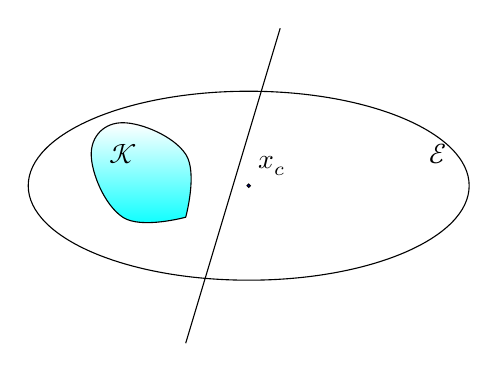
\begin{tikzpicture}[scale=0.4]
 \draw[top color=white, bottom color=cyan] plot[smooth, tension=.7] coordinates {(-3,2) (-5,2) (-6,4) (-5,5) (-3,4) (-3,2)};
 \node at (-5,4) {$\mathcal{K}$};
\draw (0,8) -- (-3,-2);
\draw [fill=qqqqff] (-1,3) circle (1.5pt) 
   node [above right] {$x_c$};
\draw  (-1,3) ellipse (7 and 3);
  \node at (5,4) {$\mathcal{E}$};
\end{tikzpicture}
\caption{Ellipsoid, feasible region, and cut}
\label{fig:ellipsoid}
\end{figure}

Updating the ellipsoid (deep-cut)

Calculation of minimum volume ellipsoid covering:
\[\mathcal{E} \cap \{z \mid g^\top (z - x_c) + \beta \leq 0 \}
\]
Let \(\tilde{g} = P\,g\), \(\tau^2 = g^\top P g\).

\begin{itemize}
\tightlist
\item
  If \(n \cdot \beta < -\tau\) (shallow cut), no smaller ellipsoid can be found.
\item
  If \(\beta > \tau\), intersection is empty.
\end{itemize}

Otherwise,
\[x_c^+ = x_c - \frac{\rho}{ \tau^2 } \tilde{g}, \qquad
  P^+ = \delta\cdot\left(P - \frac{\sigma}{ \tau^2 } \tilde{g}\tilde{g}^\top\right)
\]
where
\[\rho = \frac{ \tau+nh}{n+1}, \qquad
  \sigma = \frac{2\rho}{ \tau+\beta}, \qquad
  \delta = \frac{n^2(\tau^2 - \beta^2)}{(n^2 - 1)\tau^2}
\]

Even better, split \(P\) into two variables \(\kappa \cdot Q\).
Let \(\tilde{g} = Q \cdot g\), \(\omega = g^\top\tilde{g}\), \(\tau = \sqrt{\kappa\cdot\omega}\).
\[x_c^+ = x_c - \frac{\rho}{\omega} \tilde{g}, \qquad
  Q^+ = Q - \frac{\sigma}{\omega} \tilde{g}\tilde{g}^\top, \qquad
  \kappa^+ =  \delta\cdot\kappa
\]
Reduce \(n^2\) multiplications per iteration.
Note that:

\begin{itemize}
\tightlist
\item
  The determinant of \(Q\) decreases monotonically.
\item
  The range of \(\delta\) is \((0, \frac{n^2}{n^2 - 1})\)
\end{itemize}

\hypertarget{sec:central-cut}{%
\subsection{Central Cut}\label{sec:central-cut}}

A Special case of deep cut when \(\beta = 0\).
Deserve a separate implement because it is much simplier.
Let \(\tilde{g} = Q\,g\), \(\tau = \sqrt{\kappa\cdot\omega}\),

\[\rho = {\tau \over n+1}, \qquad
  \sigma = {2 \over n+1}, \qquad
  \delta = {n^2 \over n^2 - 1}
\]

\hypertarget{sec:parallel-cuts}{%
\subsection{Parallel Cuts}\label{sec:parallel-cuts}}

Oracle returns a pair of cuts instead of just one.
The pair of cuts is given by \(g\) and \((\beta_1, \beta_2)\) such that:
\[\begin{array}{l}
    g^\top (x - x_c) + \beta_1 \leq 0,  \\
    g^\top (x - x_c) + \beta_2 \geq 0,
  \end{array}
\]
for all \(x \in \mathcal{K}\).

Only linear inequality constraint can produce such parallel cut:
\[ l \leq a^\top x + b \leq u, \qquad L \preceq F(x) \preceq U
\]

Usually, provide faster convergence.

\begin{figure}
\hypertarget{fig:parallel_cut}{%
\centering
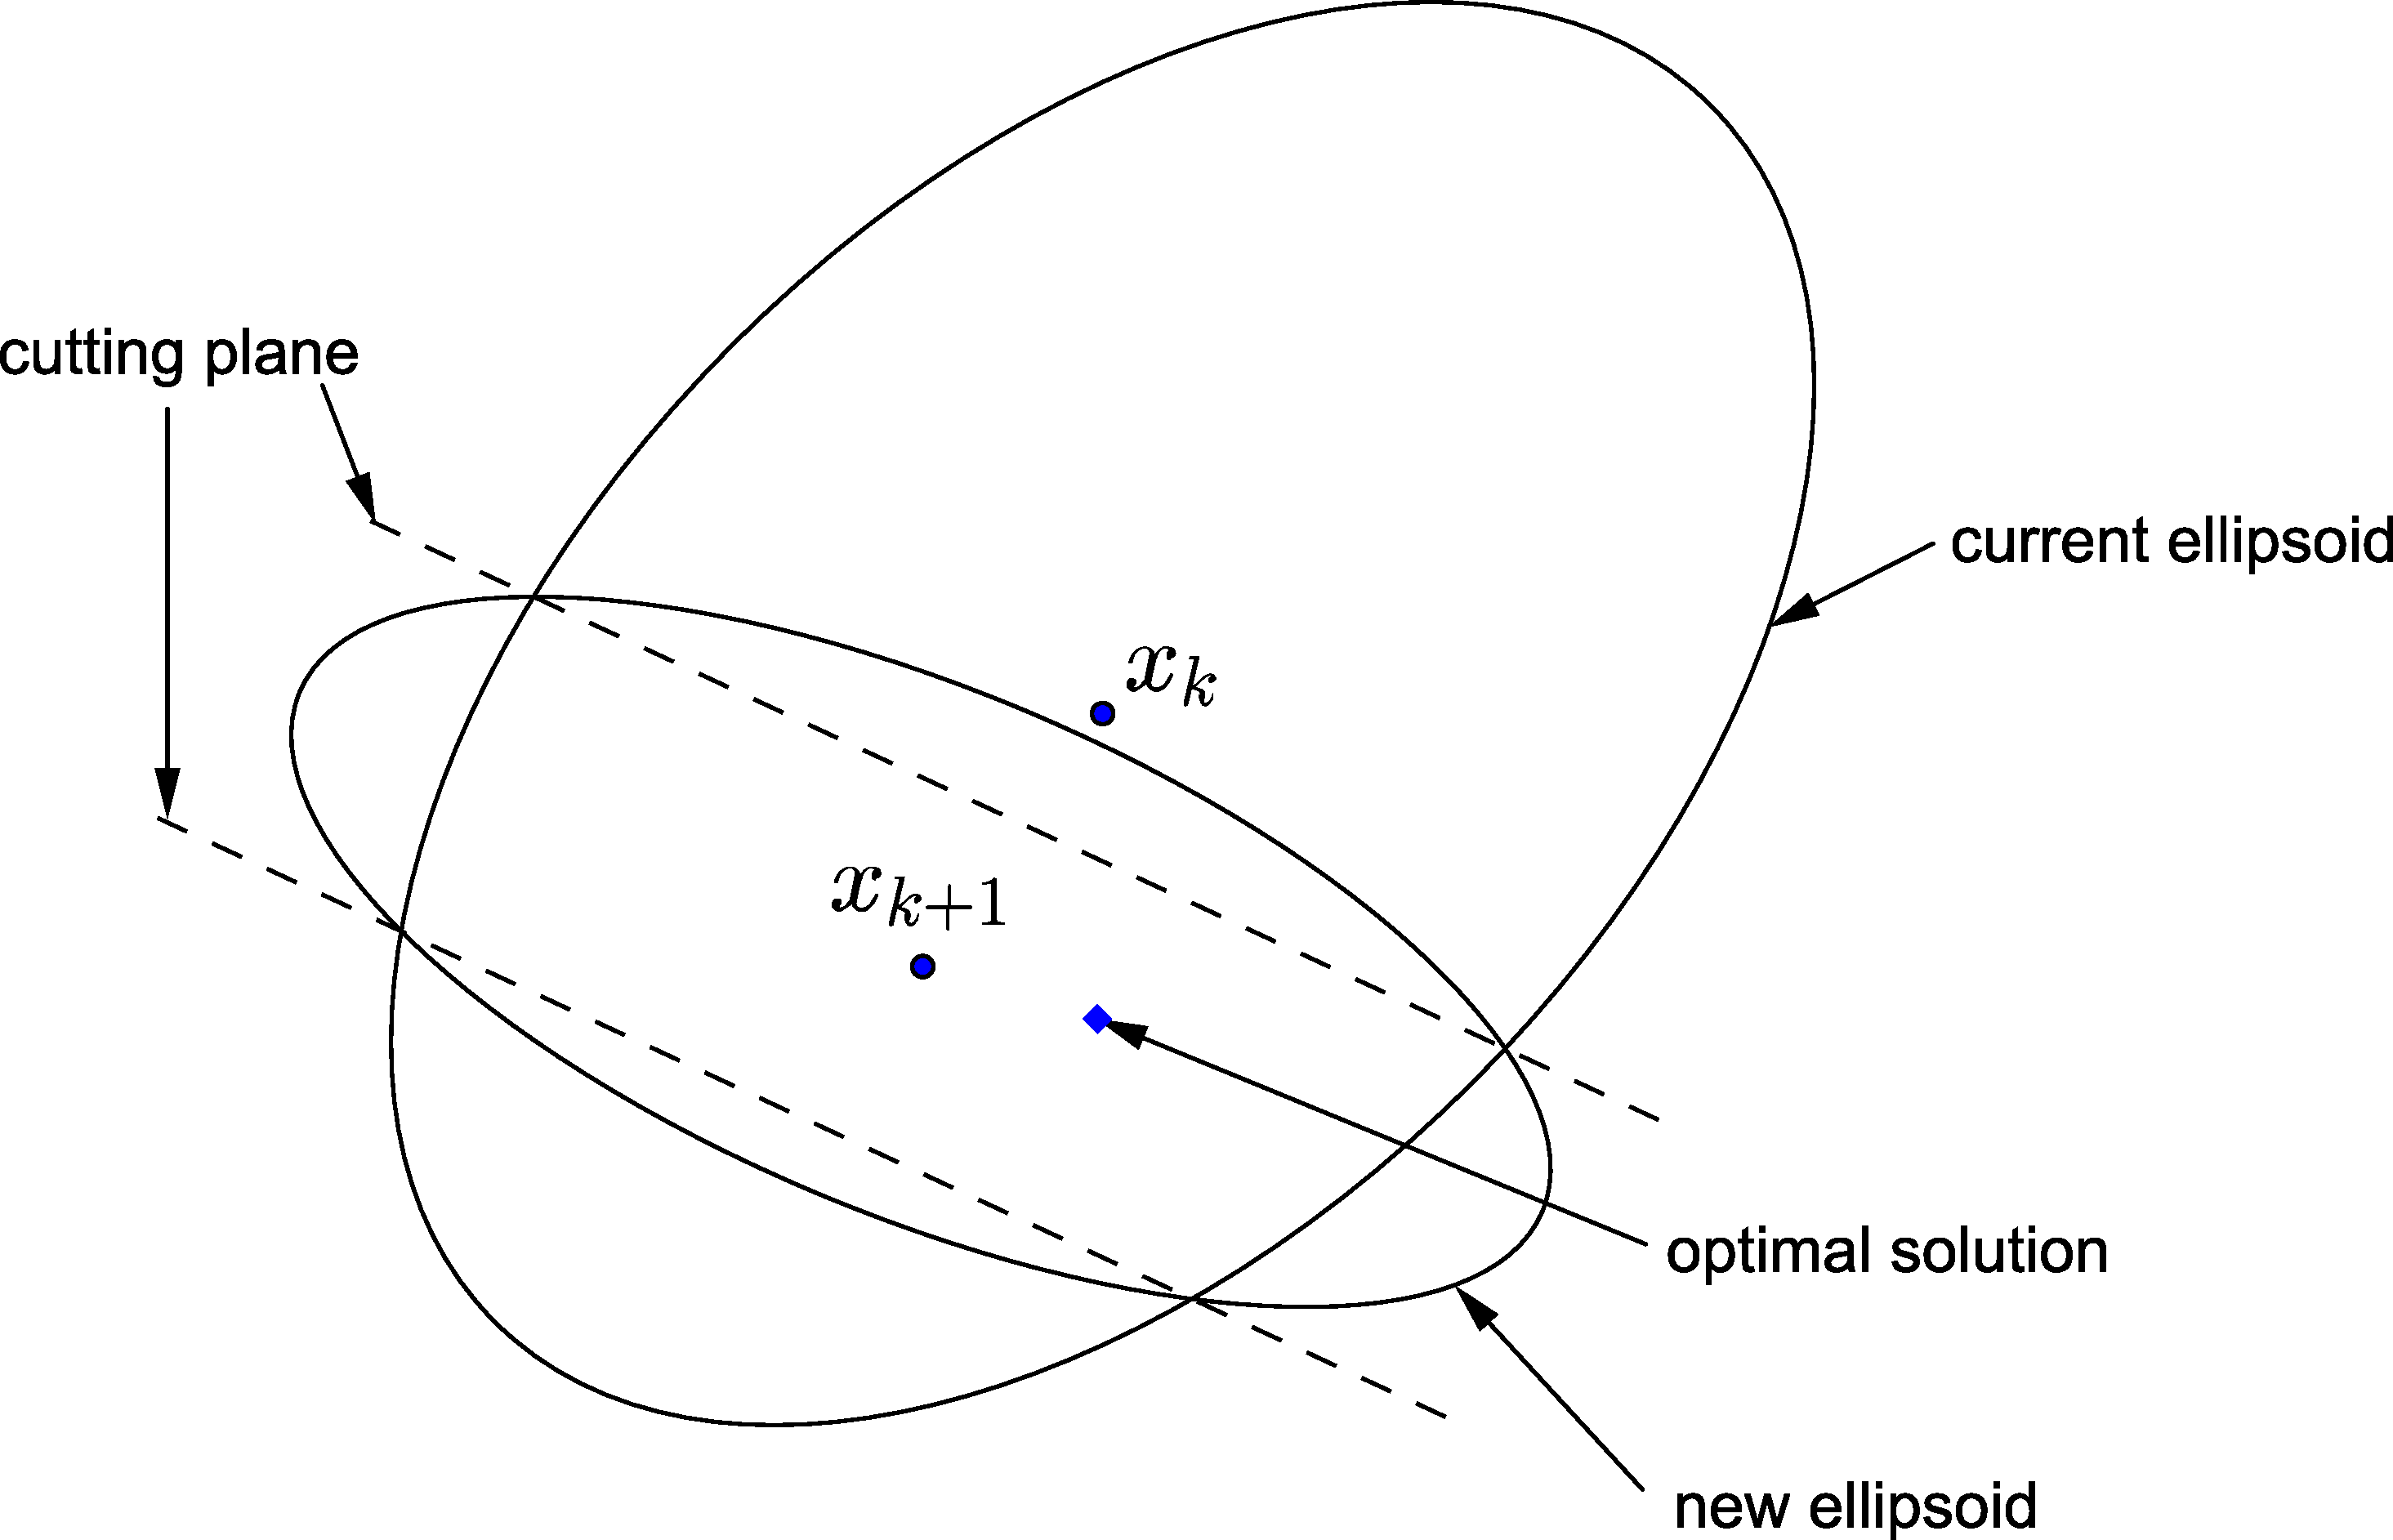
\includegraphics{ellipsoid.files/parallel_cut.pdf}
\caption{Parallel cuts}\label{fig:parallel_cut}
}
\end{figure}

Updating the ellipsoid

Let \(\tilde{g} = Q\,g\), \(\tau^2 = \kappa\cdot\omega\).

\begin{itemize}
\tightlist
\item
  If \(\beta_1 > \beta_2\), intersection is empty.
\item
  If \(\beta_1 \beta_2 < -\tau^2/n\), no smaller ellipsoid can be found.
\item
  If \(\beta_2^2 > \tau^2\), it reduces to deep-cut with \(\alpha = \alpha_1\).
\end{itemize}

Otherwise,
\[x_c^+ = x_c - \frac{\rho}{\omega} \tilde{g}, \qquad
    Q^+ = Q - \frac{\sigma}{\omega} \tilde{g}\tilde{g}^\top, \qquad
    \kappa^+ =  \delta \kappa
\]
where
\[\begin{array}{lll}
      \bar{\beta} &=& (\beta_1 + \beta_2)/2 \\
      \xi^2 &=& (\tau^2 - \beta_1^2)(\tau^2 - \beta_2^2) + (n(\beta_2 - \beta_1)\bar{\beta})^2, \\
      \sigma &=& (n + (\tau^2 - \beta_1\beta_2 - \xi)/(2\bar{\beta}^2)) / (n + 1), \\
      \rho &=& \bar{\beta}\cdot\sigma, \\
      \delta &=& (n^2/(n^2-1)) (\tau^2 - (\beta_1^2 + \beta_2^2)/2 + \xi/n) / \tau^2 .
\end{array}
\]

\hypertarget{sec:example-fir-filter-design}{%
\subsubsection{Example: FIR filter design}\label{sec:example-fir-filter-design}}

\begin{figure}
\hypertarget{fig:fir_strctr}{%
\centering
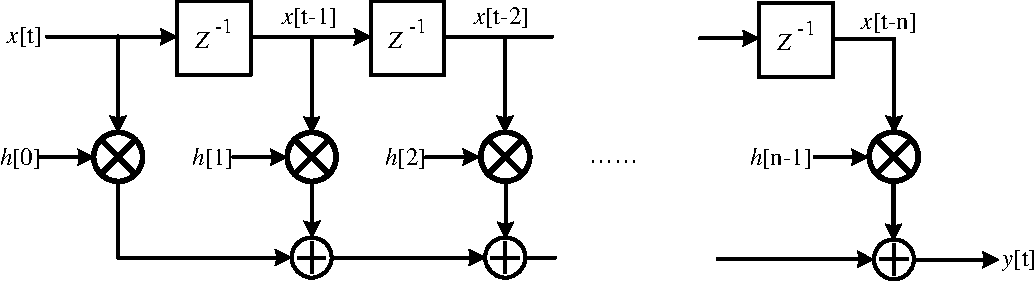
\includegraphics{ellipsoid.files/fir_strctr.pdf}
\caption{FIR filter structure}\label{fig:fir_strctr}
}
\end{figure}

The time response is:
\[ y[t] = \sum_{k=0}^{n-1}{h[k]u[t-k]}.\]
The frequency response:
\[ H(\omega)~=~\sum_{m=0}^{n-1}{h(m)e^{-jm\omega}}.\]
The magnitude constraints on frequency domain are expressed as
\[ L(\omega)~\leq~|H(\omega)|~\leq~U(\omega),~\forall~\omega\in(-\infty,+\infty),\]
where \(L(\omega)\) and \(U(\omega)\) are the lower and upper (nonnegative) bounds at frequency \(\omega\) respectively.

Note that the constraint is non-convex in general.However, via \emph{spectral factorization}, it can transform into a convex one~\citep{wu1999fir}:
\[ L^2(\omega)~\leq~R(\omega)~\leq~U^2(\omega),~\forall~\omega\in(0,\pi),
\]
where \(R(\omega)=\sum_{i=-1+n}^{n-1}{r(t)e^{-j{\omega}t}}=|H(\omega)|^2\). The vector \(\mathbf{r}=(r(-n+1),r(-n+2),...,r(n-1))\) contains the autocorrelation coefficients, which can be determined by \(\mathbf{h}\):
\[ r(t)~=~\sum_{i=-n+1}^{n-1}{h(i)h(i+t)},~t\in\mathbf{Z},
\]
where \(h(t)=0\) for \(t < 0\) or \(t > n - 1\). The whole problem can be formulated as:
\[\begin{array}{ll}
      \text{min}  & \gamma \\
      \text{s.t.} & L^2(\omega) \leq R(\omega) \leq U^2(\omega), \; 
                                    \forall \omega \in [0,\pi],   \\
                  & R(\omega) > 0, \forall \omega \in [0,\pi].
  \end{array}
\]

\begin{figure}
\hypertarget{fig:lowpass}{%
\centering
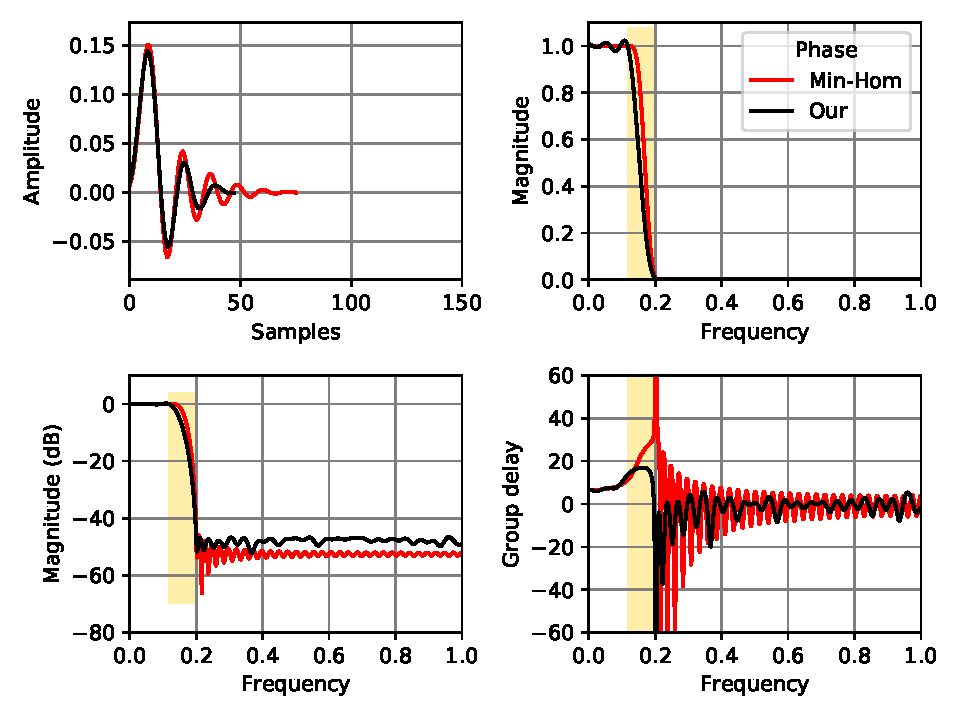
\includegraphics{ellipsoid.files/lowpass.pdf}
\caption{Result}\label{fig:lowpass}
}
\end{figure}

\hypertarget{sec:example-maximum-likelihood-estimation}{%
\subsubsection{Example: Maximum Likelihood estimation}\label{sec:example-maximum-likelihood-estimation}}

Consider
\[\begin{array}{ll}
    \min_{\kappa, p}  & \log\det(\Omega(p) + \kappa\cdot I) +
                \mathrm{Tr}((\Omega(p) + \kappa\cdot I)^{-1}Y), \\
    \text{s.t.}       & \Omega(p) \succeq 0, \kappa \geq 0 . \\
  \end{array}
\]
Note that the 1st term is concave, the 2nd term is convex. However, if there are enough samples such that \(Y\) is a positive definite matrix, then the function is convex within \([0, 2Y]\).
Therefore, the following problem is convex:
\[\begin{array}{ll}
    \min_{\kappa, p}  & \log\det V(p) + \mathrm{Tr}(V(p)^{-1}Y),\\
    \text{s.t.}       & \Omega(p) + \kappa \cdot I = V(p) \\
                      & 0 \preceq V(p) \preceq 2Y, \kappa {>} 0.
  \end{array}
\]

\hypertarget{sec:discrete-optimization}{%
\subsection{Discrete Optimization}\label{sec:discrete-optimization}}

Many engineering problems can be formulated as a convex/geometric programming, e.g.~digital circuit sizing. Yet in an ASIC design, often there is only a limited set of choices from the cell library. In other words, some design variables are discrete. The discrete version can be formulated as Mixed-Integer Convex programming (MICP) by mapping the design variables to integers.

What's wrong with the existing methods? Mostly based on relaxation. Then use the relaxed solution as a lower bound and use the branch--and--bound method for the discrete optimal solution. Note that the branch-and-bound method does not utilize the convexity of the problem. What if I can only evaluate constraints on discrete data?Workaround: convex fitting?

Consider:
\[\begin{array}{ll}
        \text{minimize}      & f_0(x), \\
        \text{subject to}    & f_j(x) \leq 0, \; \forall j=1,2,\ldots, \\
                             & x \in \mathbb{D},
  \end{array}
\]
where \(f_0(x)\) and \(f_j(x)\) are ``convex''. Note that some design variables are discrete. The oracle looks for the nearby discrete solution \(x_d\) of \(x_c\) with the cutting-plane:
\[ g^\top (x - x_d) + \beta \leq 0, \beta \geq 0, g \neq 0.
\]
Note that the cut may be a shallow cut. Suggestion: use different cuts as possible for each iteration (e.g.~round-robin the evaluation of constraints).

\begin{figure}
\hypertarget{fig:lowpass_ripple}{%
\centering
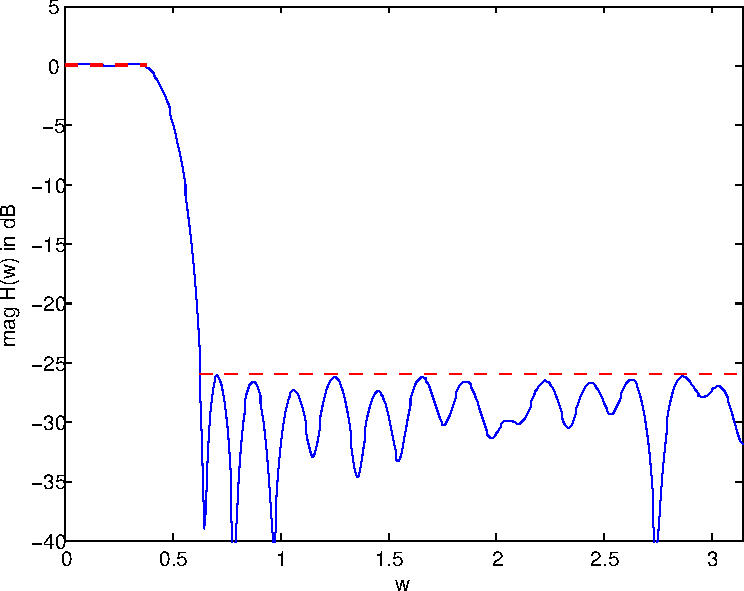
\includegraphics{ellipsoid.files/lowpass_ripple.pdf}
\caption{Lowpass ripple}\label{fig:lowpass_ripple}
}
\end{figure}

\renewcommand\refname{References}
\bibliography{fir-ref.bib}

\end{document}
